% LaTeX Präsentationsvorlage (2013) der TU Graz, rev12, 2013/01/31
\documentclass{beamer}
% \documentclass[aspectratio=169]{beamer}
\usetheme{tugraz2013}
% \usetheme[notes]{tugraz2013}
% \usetheme[minimal]{tugraz2013}

%% Titelblatt-Einstellungen
\title[Android Bluetooth Credential Store]{Android Bluetooth \\ Credential Store}
\author{Camilla Reis}
% \date{Graz, XX. Dezember 2010}		% \today für heutiges Datum verwenden
\date{Graz, 7. November 2018}
\institute[IAIK]{\\ Institute of Applied Information Processing and Communications}
\instituteurl{www.tugraz.at}
% \institutelogo{kurz.pdf}
% \additionallogo{institutslogo.pdf}

%% Präsentationszeit: 15-20min 

\usepackage{hyperref}
\def\UrlBreaks{\do\/\do-}

%%%%%%%%%%%%%%%%%%%%%%%%%%%%%%%%%%%%%%%%%%%%%%%%%%%%%%%%%%%%%%%%%%%%%%%%%%%%
\begin{document}
%%%%%%%%%%%%%%%%%%%%%%%%%%%%%%%%%%%%%%%%%%%%%%%%%%%%%%%%%%%%%%%%%%%%%%%%%%%%
\titleframe

\begin{frame}
	\centering
	\vfill
	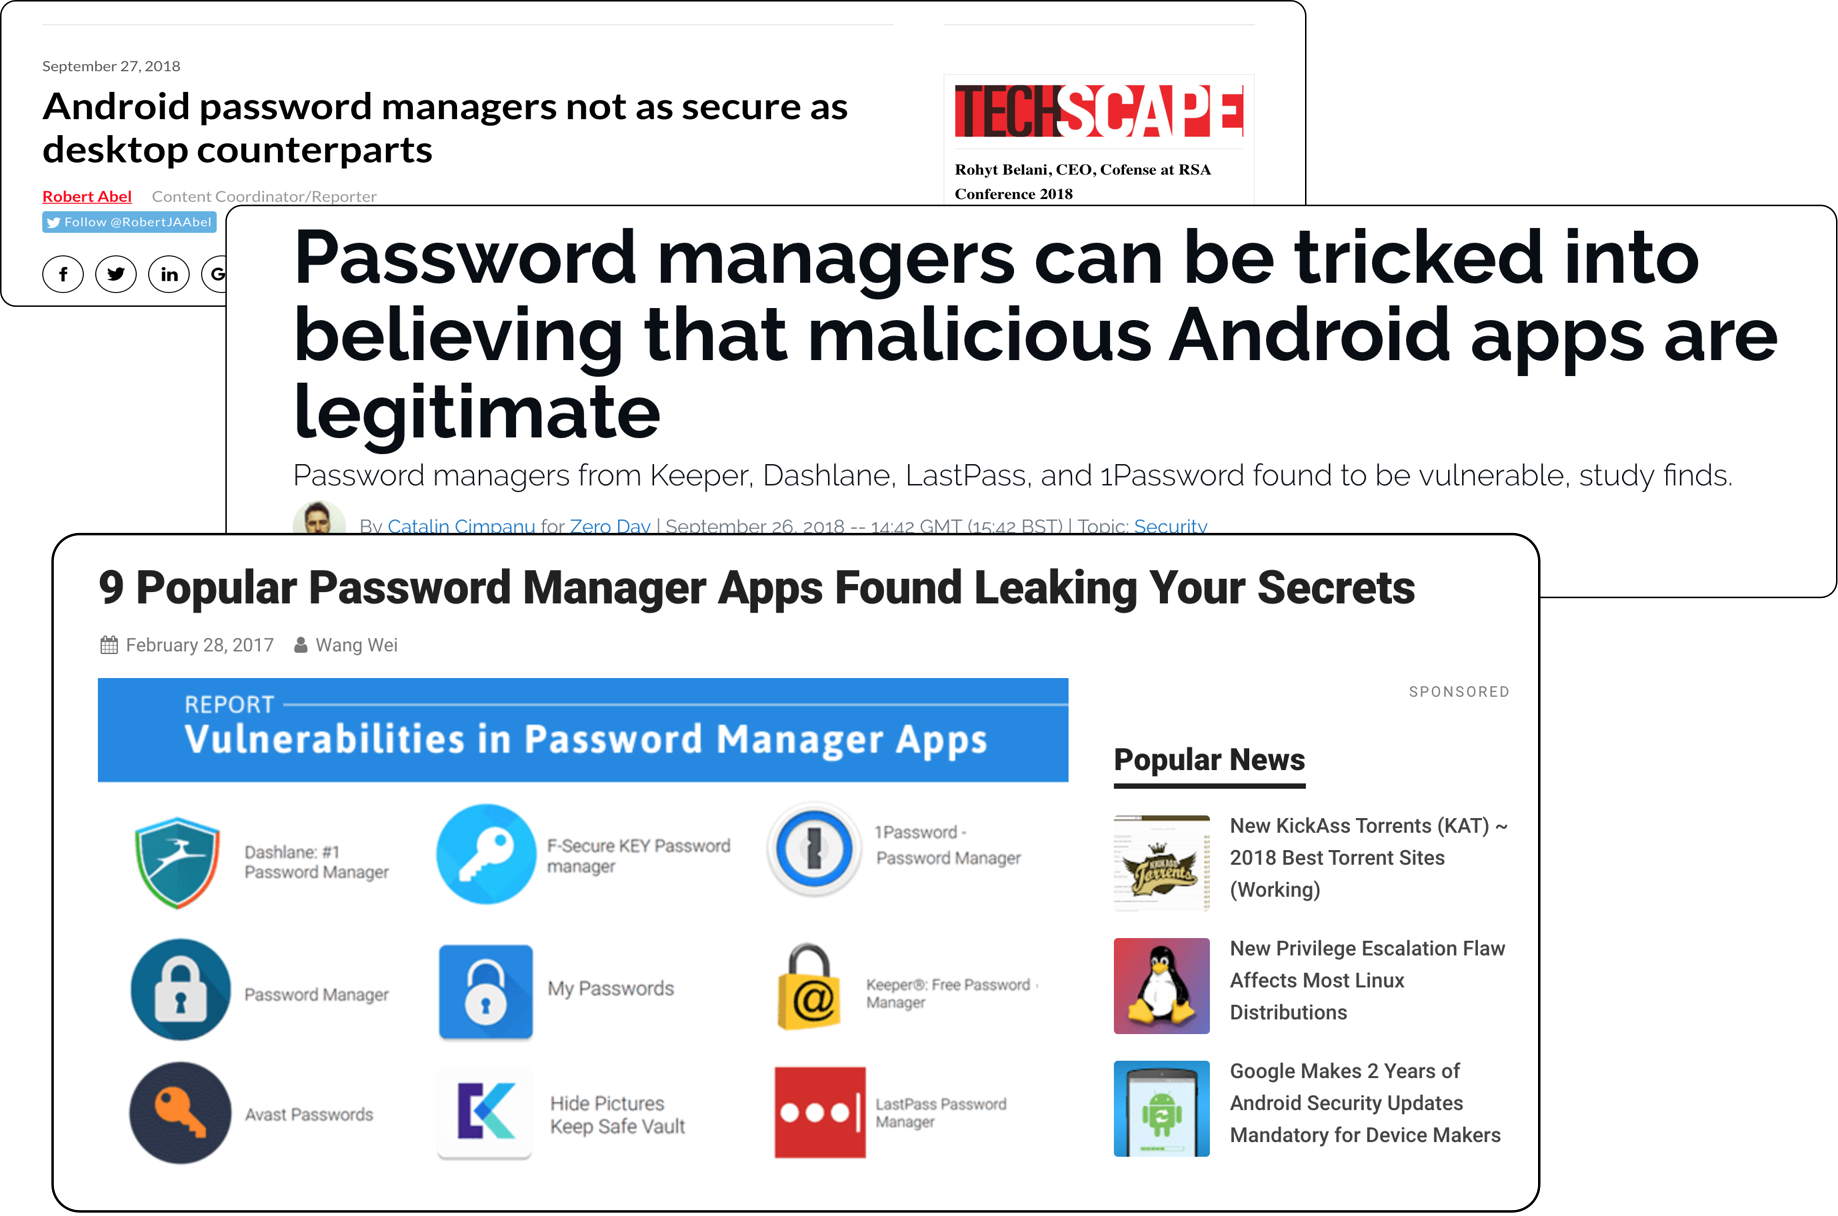
\includegraphics[width=1\textwidth]{images/papers.png}
	\vfill
\end{frame}


\section{Motivation}
\begin{frame}{Existing Solutions}
	\begin{itemize}
		\item Android applications prone to phishing attacks.
		\item Master passwords stored in plain text.
		\item Sniffing data from uncleaned clipboard.
		\item Web-based password managers use cookies for authentication.
	\end{itemize}
\end{frame}


\begin{frame}{Motivation of Project}
\vspace{-5mm}
\begin{itemize}
	\item The Android platform offers
	\begin{itemize}
		\item Trusted Execution Environment (TEE)
		\item Biometric authentication methods
		\item Sandboxing
	\end{itemize}
	\item Smartphones support our everyday life.
\end{itemize}
\end{frame}

\begin{frame}{Motivation of Project}
\vspace{-5mm}
\begin{itemize}
	\item Availability of credentials is important.
	\item Third parties compromise confidentiality.
	\item Our goal is to
	\begin{itemize}
		\item provide secure storage and availability of credentials.
		\item reduce external dependencies to increase confidentiality.
	\end{itemize}
\end{itemize}
\end{frame}




%\begin{frame}{Motivation of Project}
%\vspace{-5mm}
%\begin{itemize}
%	\item Our goal is to
%	\begin{itemize}
%		\item provide secure storage and availability of credentials.
%		\item reduce external dependencies to increase confidentiality.
%	\end{itemize}
%\end{itemize}
%\end{frame}


\begin{frame}{Motivation of Project}
\begin{itemize}
	\item Solution:
	\begin{itemize}
		\item Android credential manager 
		\item Google Chrome extension
		\item Bluetooth LE connection for data exchange
		\item Data is stored on device
		\item Authentication is done via fingerprint
	\end{itemize}
\end{itemize}
\end{frame}


%%%%%%%%%%%%%%%%%%%%%%%%%%%%%%%%%%%%%%%%%%%%%%%%%%%%%%%%%%%%%%%%%%%%%%%%%%%%

\section{Architecture of Project}

\begin{frame}{Workflow of Devices}
\vspace{-3mm}
\centering
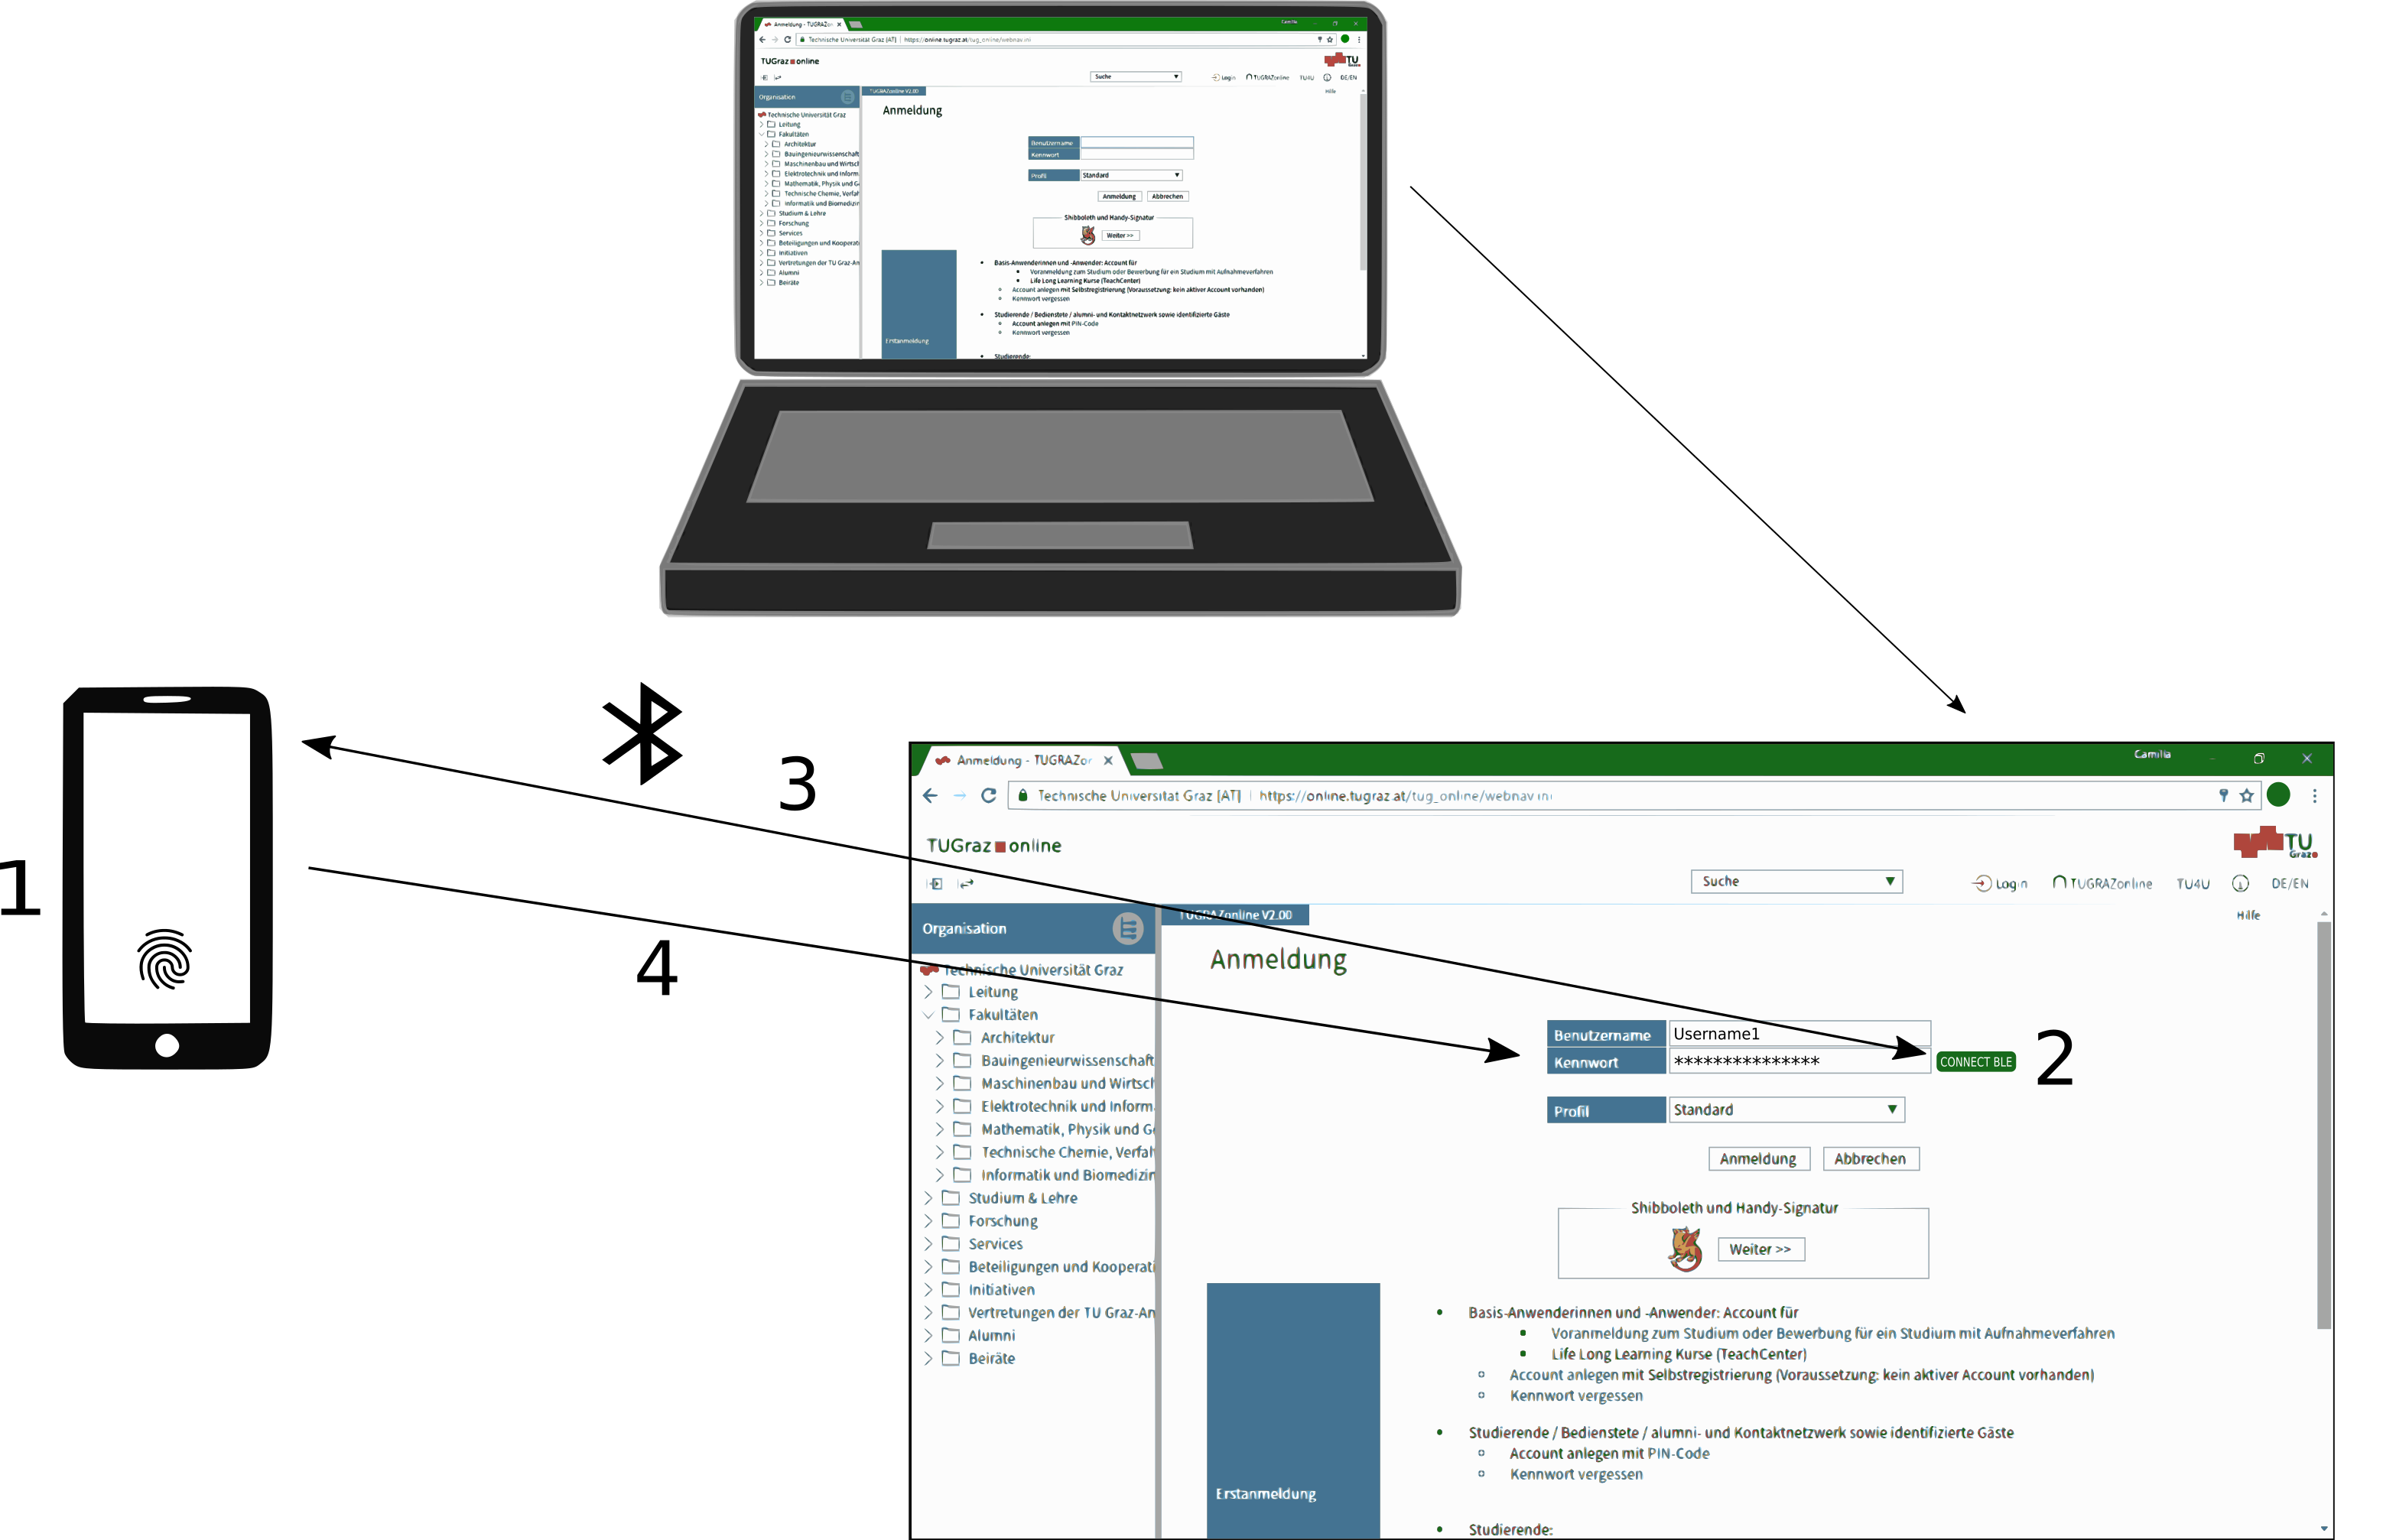
\includegraphics[width=0.9\textwidth]{images/Communication.png}
\end{frame}


\begin{frame}[shrink=8]{Requirements}
\begin{columns}[onlytextwidth]
	\begin{column}{0.45\textwidth}
		Application requirements:
		\begin{itemize}
			\item Storage and management of credentials
			\item En- and decryption
			\item Authentication through biometrics
		\end{itemize}
	\end{column}
	\begin{column}{0.47\textwidth}
		Extension requirements:
		\begin{itemize}
			\item Injection of a button
			\item Establishing BLE connection
			\item Read and insert characteristics
		\end{itemize}
	\end{column}
\end{columns} 
\end{frame}


\begin{frame}{Storage of Credentials}
\vspace{-10mm}
	\begin{columns}[onlytextwidth]
		\begin{column}{0.7\textwidth}
			\begin{itemize}
				\item ORM greenDAO
				\begin{itemize}
					\item Handles storing, deleting, updating tasks.
				\end{itemize}
				\item Database lies in persistent memory.
				\item Only application can access data.
			\end{itemize}
		\end{column}
		\begin{column}{0.3\textwidth}
			\begin{center}
			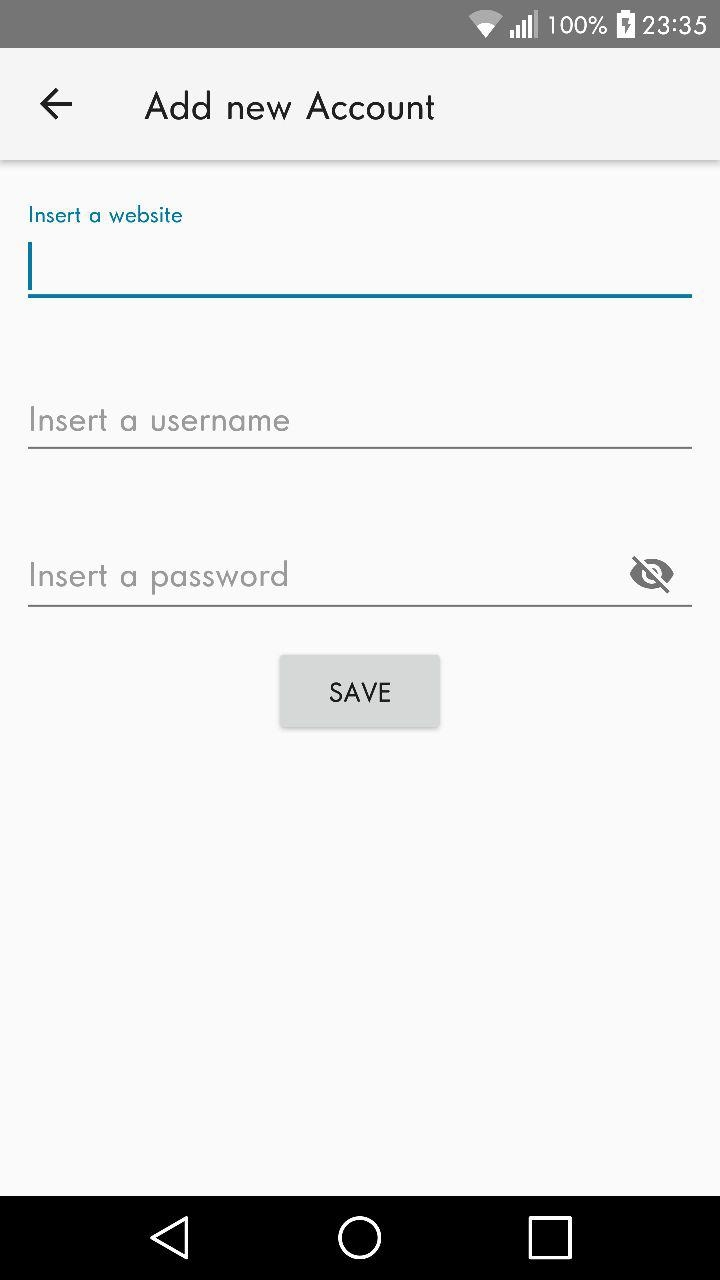
\includegraphics[width=0.8\textwidth]{images/AddAccountActivity.jpg} \\
			\end{center}
		\end{column}
	\end{columns}
\end{frame}


\begin{frame}{Encryption of Credentials}
\vspace{-5mm}
\begin{itemize}
	\item Symmetric key encryption algorithm AES-GCM:
	\begin{itemize}
		\item No distribution of public key component.
		\item Fast execution of computations.
		\item Consumes fewer resources.
		\item GCM provides confidentiality, integrity, and authenticity.
	\end{itemize} 
\end{itemize}
\end{frame}


\begin{frame}{Storage of Cryptographic Key}
\vspace{-5mm}
	\begin{itemize}
	\item AndroidKeystore stores cryptographic keys.
	\item Only application that created key can access it.
	\item Key is stored in Trusted Execution Environment (TEE).
		\begin{itemize}
		\item TEE depends on device manufacturer.
		\item Data cannot be extracted from the TEE.
		\end{itemize}
\end{itemize}
\end{frame}


\begin{frame}{Authentication through Biometrics}
\vspace{-10mm}
	\begin{columns}[onlytextwidth]
		\begin{column}{0.7\textwidth}
			\begin{itemize}
			\item Authentication via fingerprint when: 
			\begin{itemize}
				\item Accessing credentials
				\item Sending credentials
			\end{itemize}
			\item Protection of unintentional distribution.
			\end{itemize}
		\end{column}
		\begin{column}{0.3\textwidth}
			\begin{center}
			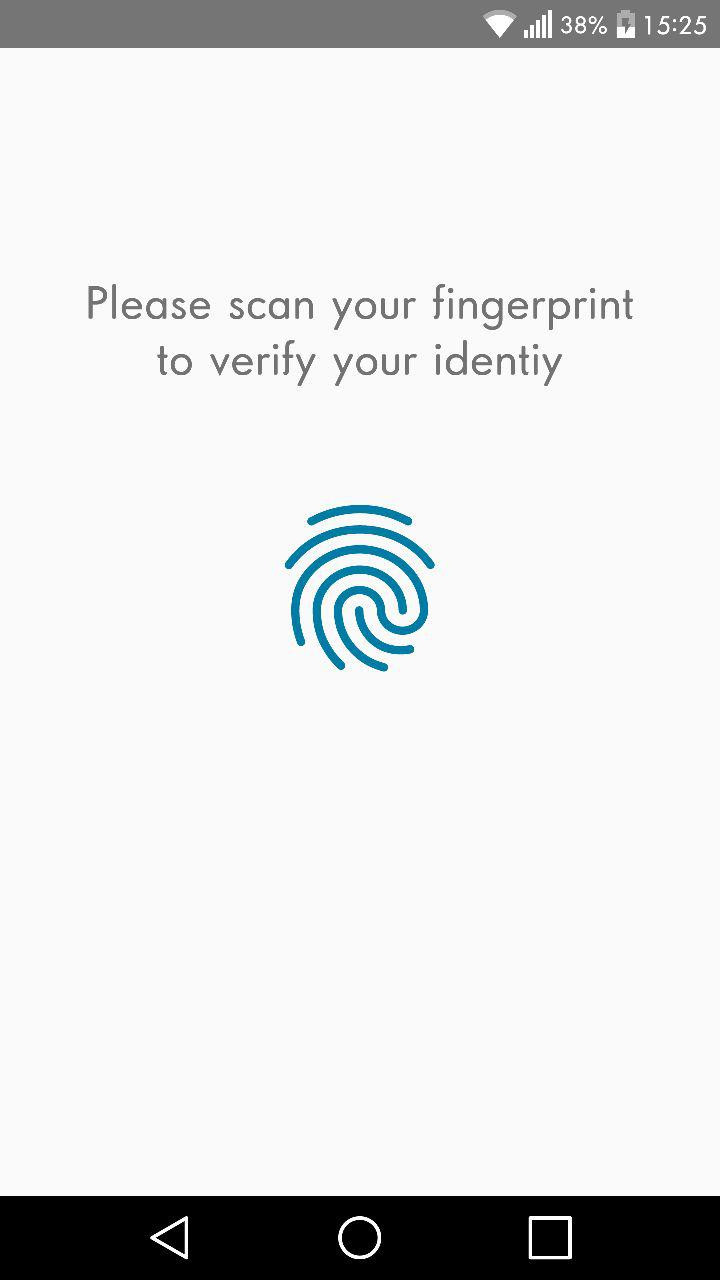
\includegraphics[width=0.8\textwidth]{images/AuthenticationScreenNew.jpg} \\
			\end{center}
		\end{column}
	\end{columns}
\end{frame}


\begin{frame}{Chrome Browser Extension}
\begin{itemize}
	\item Establish connection with BLE device.
	\item Extension acts as client and receives data.
	\item Insert data into forms.
	\item Modification of DOM.
\end{itemize}
\end{frame}


\begin{frame}{}
\vfill
\centering
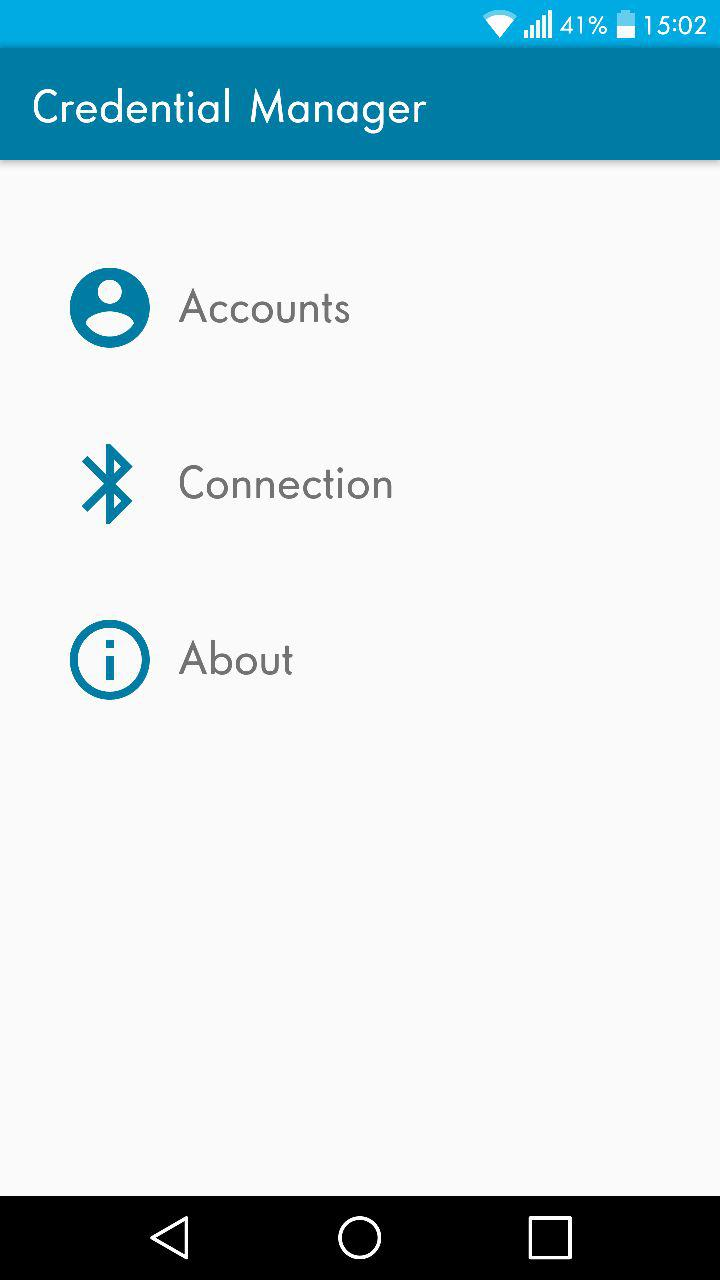
\includegraphics[width=0.31\textwidth]{images/MainActivityNew.jpg}
\hspace{0.1cm}
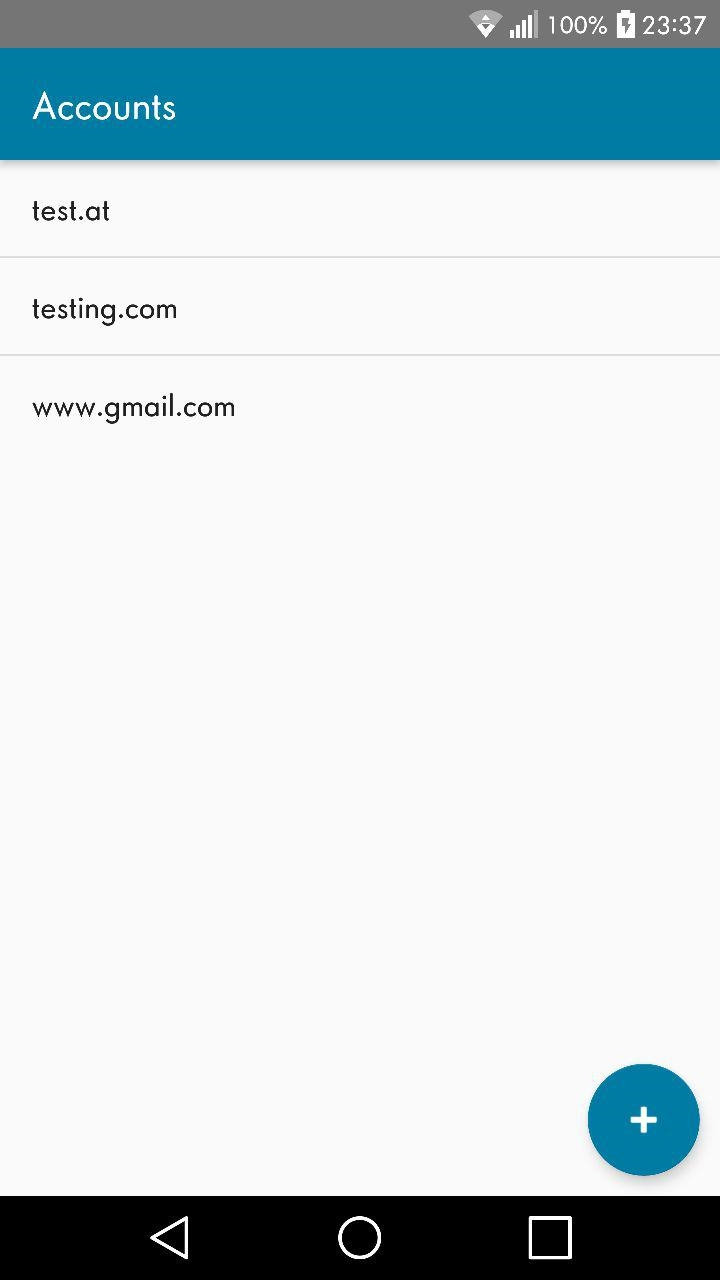
\includegraphics[width=0.31\textwidth]{images/ShowAccountsActivity.jpg}
\hspace{0.1cm}
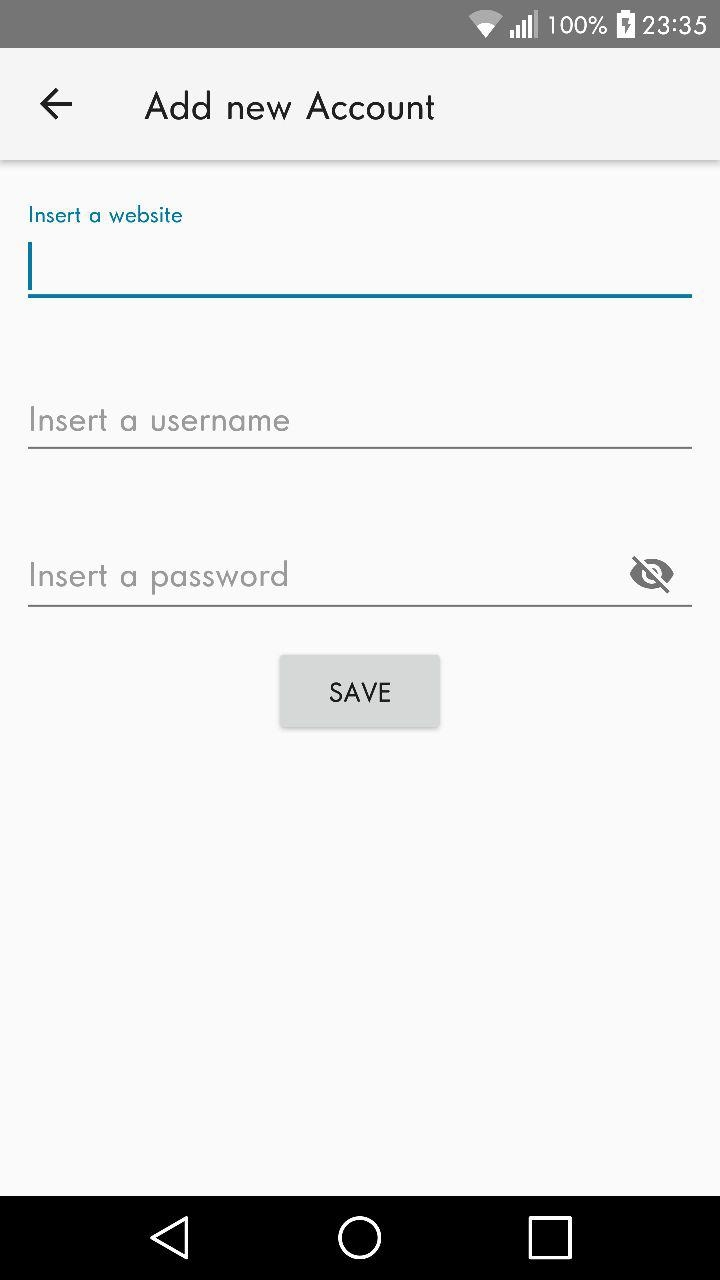
\includegraphics[width=0.31\textwidth]{images/AddAccountActivity.jpg}
\vfill
\end{frame}


\begin{frame}{}
\vfill
\centering
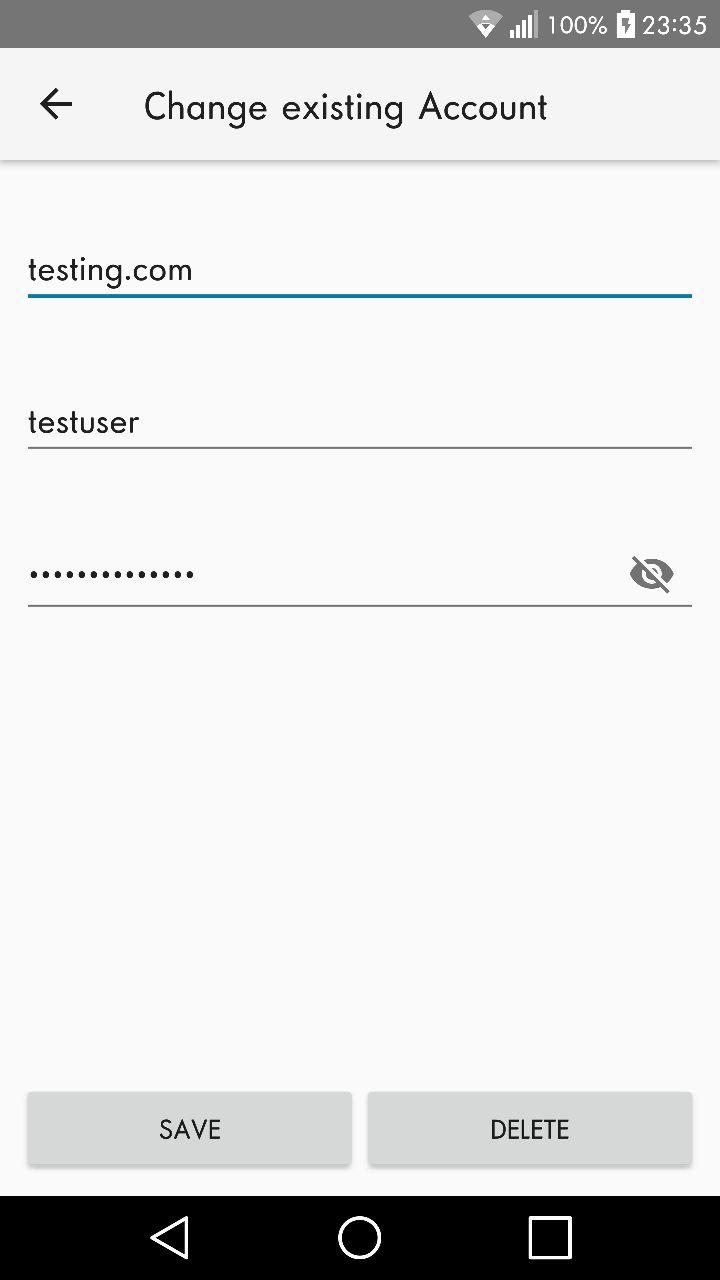
\includegraphics[width=0.31\textwidth]{images/ChangeAccountActivity.jpg}
\hspace{1cm}
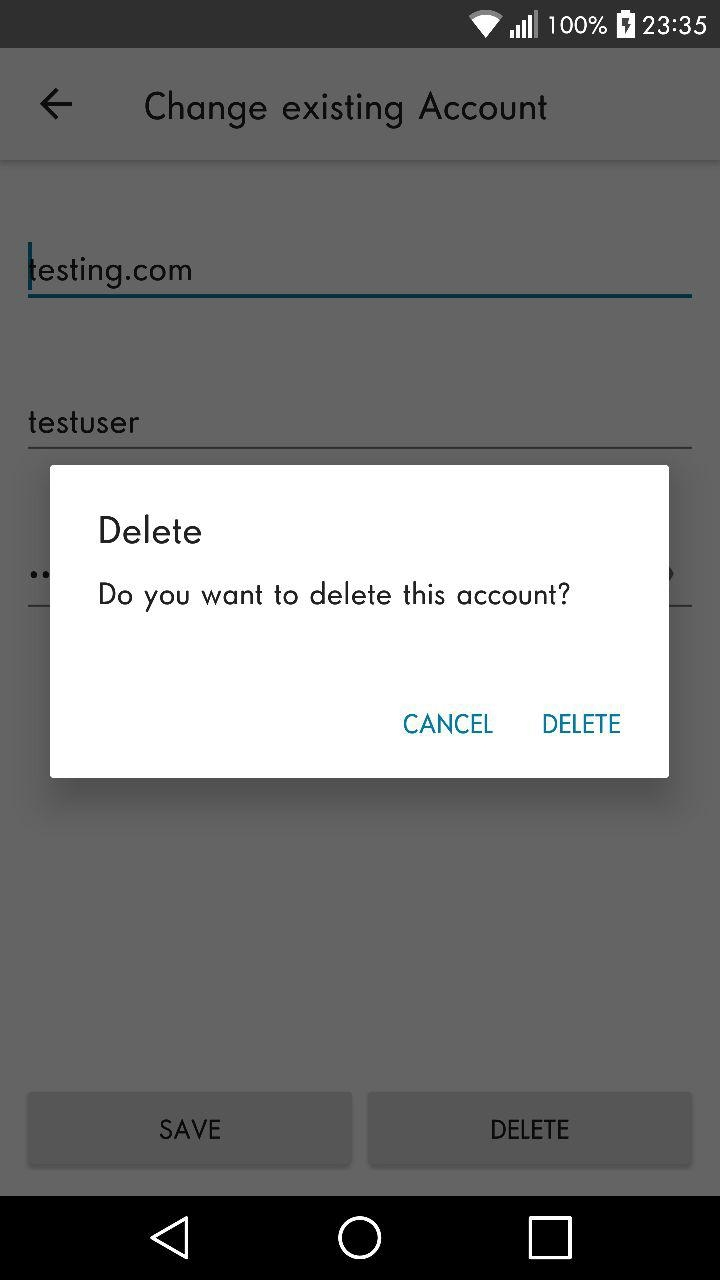
\includegraphics[width=0.31\textwidth]{images/DeleteAccount.jpg}
\vfill
\end{frame}

\begin{frame}{}
\vfill
\centering
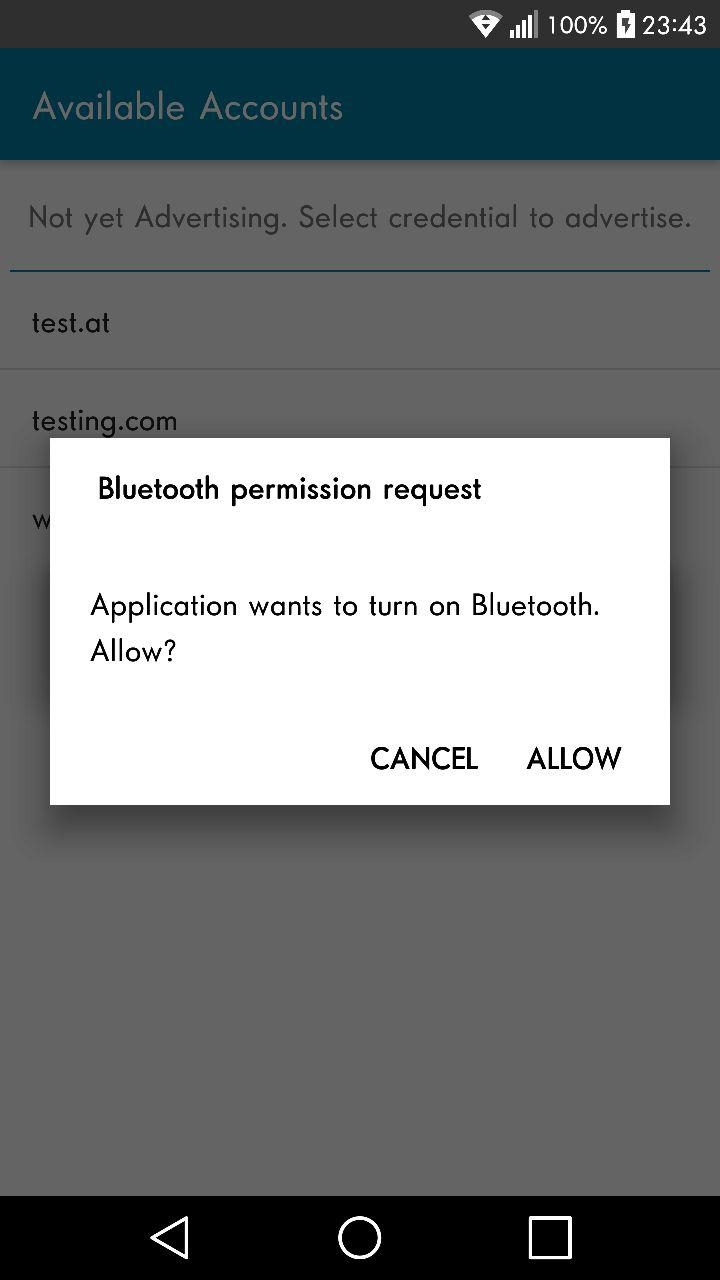
\includegraphics[width=0.31\textwidth]{images/BT_english.jpg}
\hspace{0.1cm}
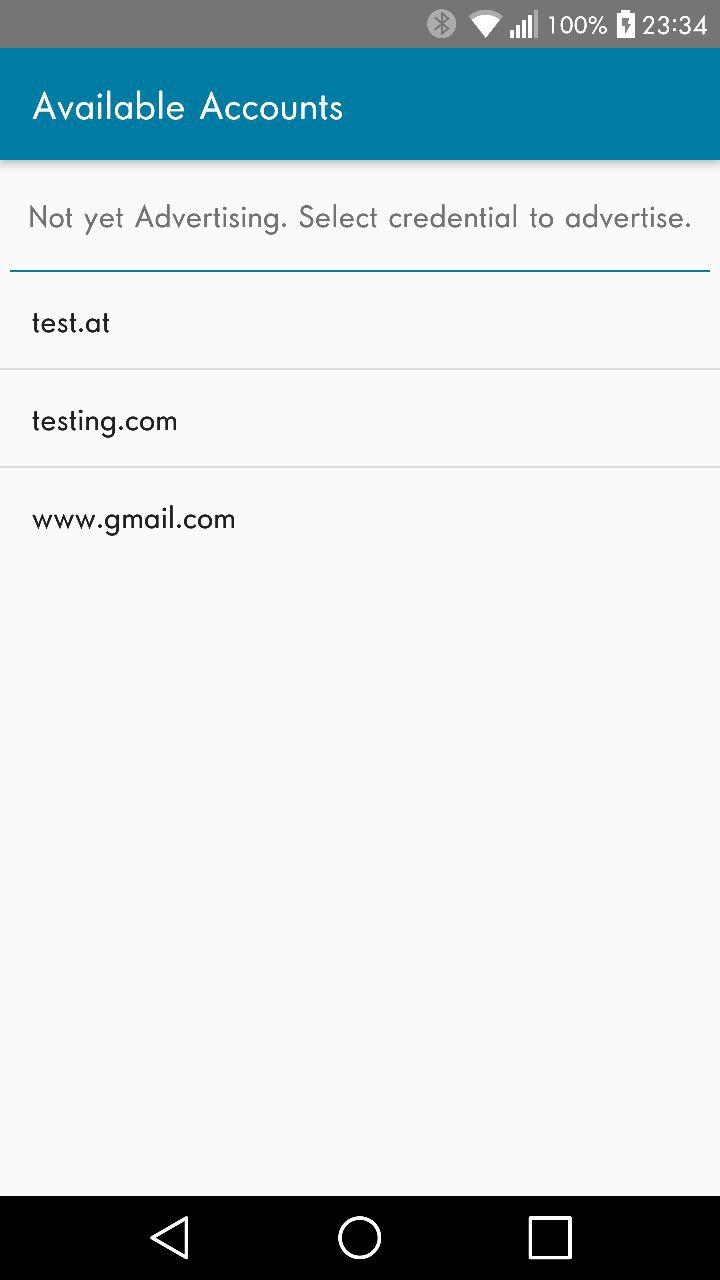
\includegraphics[width=0.31\textwidth]{images/AvailableAccounts.jpg}
\hspace{0.1cm}
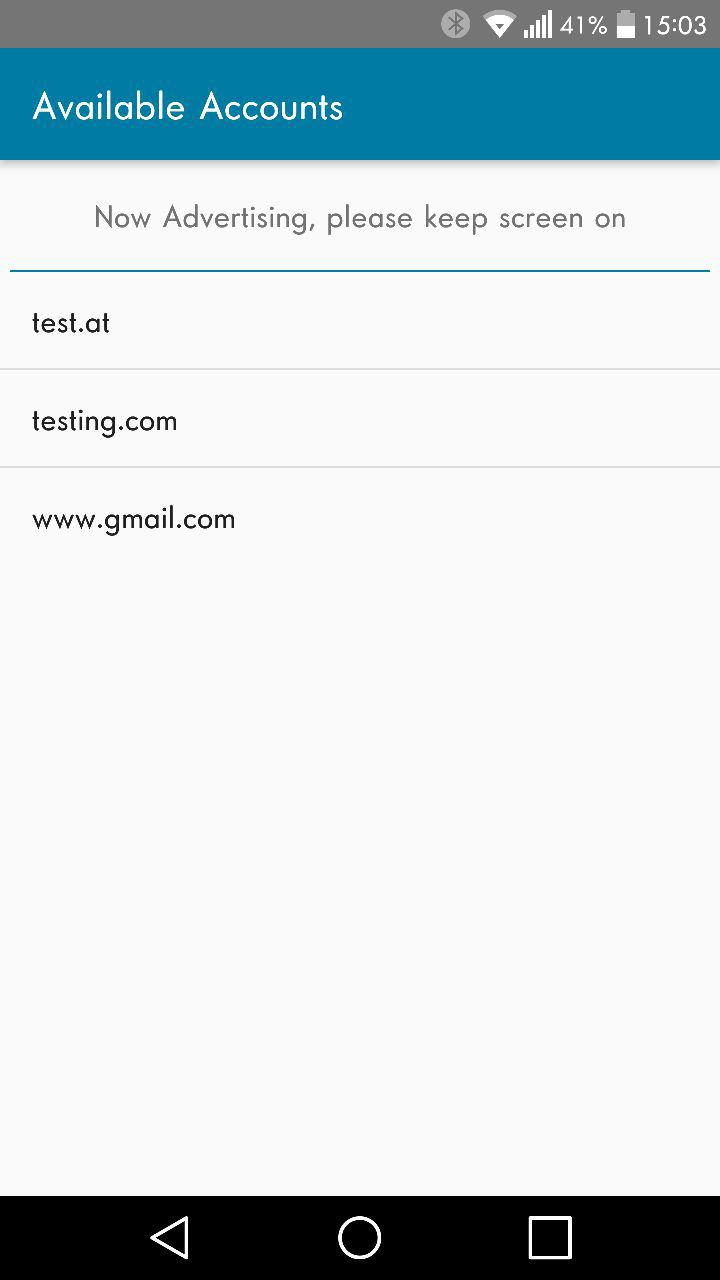
\includegraphics[width=0.31\textwidth]{images/NowAdvertising.jpg}

\vfill
\end{frame}

\begin{frame}{}
\vfill
\centering
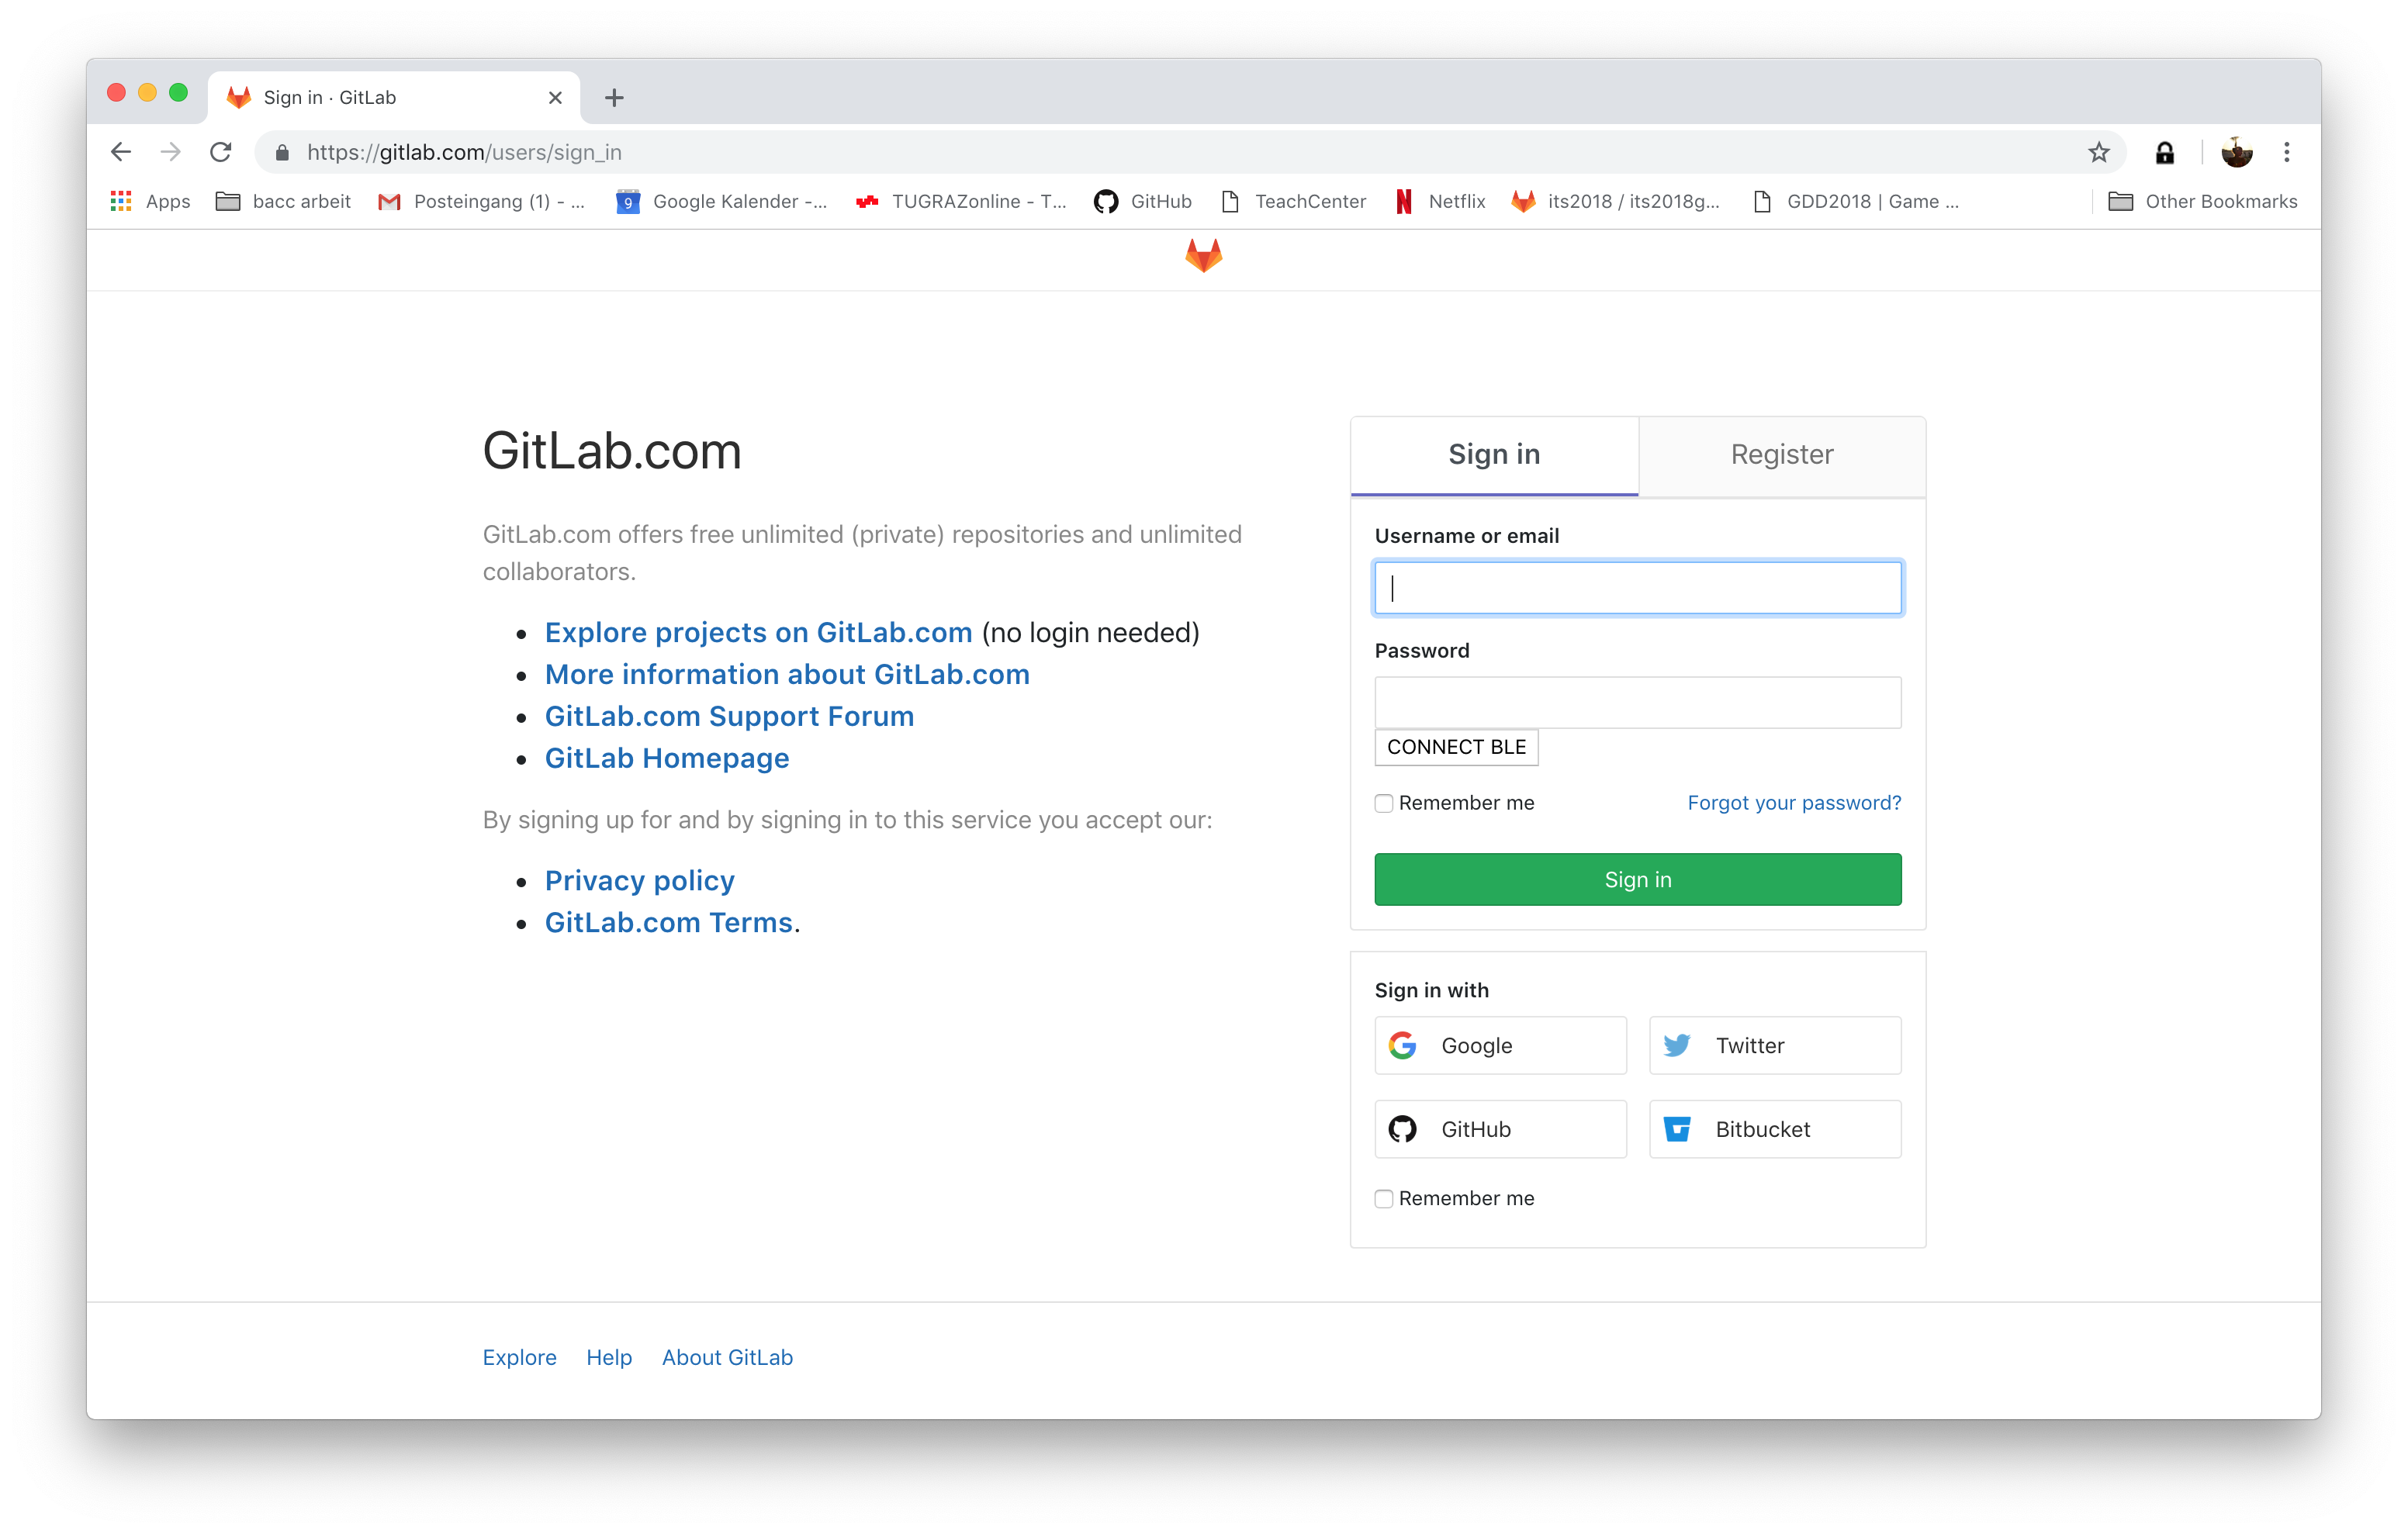
\includegraphics[width=\textwidth]{images/web.png}
\vfill
\end{frame}

\section{}
\begin{frame}\frametitle{Summary}
\begin{itemize}
	\item Reduce the risk of unauthorized access by eliminating external dependencies.
	\item Provide availability through a BLE connection.
	\item Securely store credentials on the device.
	\item Authenticate through fingerprint.
\end{itemize}
\end{frame}


%%%%%%%%%%%%%%%%%%%%%%%%%%%%%%%%%%%%%%%%%%%%%%%%%%%%%%%%%%%%%%%%%%%%%%%%%%%%

\section*{}
\begin{frame}[shrink=50]{References}
\vspace{-15mm}
\begin{enumerate}
	\item R.Abel, “Android password managers not as secure as desktop counterparts.“ https://www.scmagazine.com/home/security-news/android-password-managers-not-as-secure-as-desktop-counterparts/, 2018 \\
	\item C. Cimpanu, “Password managers can be tricked into believing that malicious Android apps are legitimate“ https://www.zdnet.com/article/password-managers-can-be-tricked-into-believing-that-malicious-android-apps-are-legitimate/, 2018 \\
	\item W. Wei, “9 Popular Password Manager Apps Found Leaking Your Secrets“ https://thehackernews.com/2017/02/password-manager-apps.html, 2017 \\
	\item F. Beaufort, “Interact with Bluetooth devices on the Web.” https://developers.google.com/web/updates/2015/07/interact- with-ble-devices-on-the-web, 2018. \\
	\item U. Ries, “Btlejack: Neues Gratis-Tool zum Belauschen von Bluetooth- Verbindungen.” https://www.heise.de/security/meldung/ Btlejack-Neues-Gratis-Tool-zum-Belauschen-von-Bluetooth- Verbindungen-4134142.html, 2018. \\
	\item Y. Haider, S. Selvan, “Confidentiality Issues in Cloud Computing and Countermeasures: A Survey“, 2016. \\
	\item GreenDAO, “greenDAO: Android ORM for your SQLite database.” http://greenrobot.org/greendao/, 2016. \\
	\item Z. Li, W. He, D. Akhawe, and D. Song, “The Emperor’s New Password Manager: Security Analysis of Web-based Password Managers,” in Proceedings of the 23rd USENIX Security Symposium, 2014. \\
\end{enumerate}
\end{frame}

%%%%%%%%%%%%%%%%%%%%%%%%%%%%%%%%%%%%%%%%%%%%%%%%%%%%%%%%%%%%%%%%%%%%%%%%%%%%

%\section{Motivation}
%%--------------------
%\begin{frame}
%\frametitle{Ziele der ersten Vorlesung}
%Einführung in die KORE
%\begin{itemize}
%	\item Geschichte der KORE kennen lernen
%	\item Aufgaben der KORE und Einordnung in das betriebliche Rechnungswesen verstehen
%	\item Wertebenen im Rechnungswesen unterscheiden
%\end{itemize}
%
%Grundlagen der KORE
%\begin{itemize}
%	\item Kostenwürfel als Hilfsmittel verwenden
%	\item Überleitung von externem zu internem Rechnungswesen durchführen
%\end{itemize}
%\end{frame}

%%%%%%%%%%%%%%%%%%%%%%%%%%%%%%%%%%%%%%%%%%%%%%%%%%%%%%%%%%%%%%%%%%%%%%%%%%%%

%\section{Related Work}
%%--------------------
%\begin{frame}
%\frametitle{Titel der Folie\\maximal zwei Zeilen}
%Text Ebene 1
%\begin{itemize}
%	\item Zweite Ebene
%	\begin{itemize}
%		\item Dritte Ebene
%		\begin{itemize}
%			\item Vierte Ebene
%		\end{itemize}
%	\end{itemize}
%\end{itemize}
%\end{frame}

%%%%%%%%%%%%%%%%%%%%%%%%%%%%%%%%%%%%%%%%%%%%%%%%%%%%%%%%%%%%%%%%%%%%%%%%%%%%

%\section{Finished Project}
%%--------------------
%\begin{frame}[fragile]
%	\frametitle{Android Application}
%	\begin{spacing}{1}
%	\begin{semiverbatim}
%SUCHE (A,x)
%1: i = 0
%2: WHILE i<n
%3:     i = i+1
%4:     \alert{IF A[i]=x THEN RETURN i}
%5: ELSE RETURN -1
%	\end{semiverbatim}
%	\end{spacing}
%\end{frame}

%%%%%%%%%%%%%%%%%%%%%%%%%%%%%%%%%%%%%%%%%%%%%%%%%%%%%%%%%%%%%%%%%%%%%%%%%%%%

%\section{Spalten und Grafiken}
%%--------------------
%\begin{frame}
%	\frametitle{Zwei Inhalte Links/Rechts\\Wahlweise Text/Grafik}
%	\begin{columns}[onlytextwidth]
%		\begin{column}{0.5\textwidth}
%			\begin{itemize}
%				\item Lorem ipsum dolor sit amet, consectetur 
%				\item adipisicing elit, sed do eiusmod tempor 
%				\item incididunt ut labore et dolore magna aliqua. 
%				\item Ut enim ad minim veniam, quis nostrud 
%			\end{itemize}
%		\end{column}
%		\begin{column}{0.5\textwidth}
%			\begin{center}
%			
\includegraphics[width=0.5\textwidth]{logo.pdf}\\
%			Grafik in Spalte 2
%			\end{center}
%		\end{column}
%	\end{columns}
%\end{frame}
%
%\section{Weitere Beispielfolien}
%
%\begin{frame}
%\frametitle{Titel der Folie\\maximal zwei Zeilen}
%	Ein Link:
%	\begin{center}
%		\url{http://www.tugraz.at}		
%	\end{center}
%\end{frame}
%
%\sectionheader[Untertitel]{Abschnittsbeginn}

%%%%%%%%%%%%%%%%%%%%%%%%%%%%%%%%%%%%%%%%%%%%%%%%%%%%%%%%%%%%%%%%%%%%%%%%%%%%

%\section{Zusammenfassung}
%%--------------------
%\begin{frame}
%	\frametitle{Zusammenfassung}
%	\begin{itemize}
%		\item Punkt 1
%		\item Punkt 2
%		\item Punkt 3
%	\end{itemize}
%\end{frame}

%%%%%%%%%%%%%%%%%%%%%%%%%%%%%%%%%%%%%%%%%%%%%%%%%%%%%%%%%%%%%%%%%%%%%%%%%%%%
\end{document}
%%%%%%%%%%%%%%%%%%%%%%%%%%%%%%%%%%%%%%%%%%%%%%%%%%%%%%%%%%%%%%%%%%%%%%%%%%%%

%% EOF
